\documentclass{article}
\usepackage{graphicx} % Required for inserting images

\title{Homework 6}
\author{Ayman Tawaalai}
\date{February 2024}

\begin{document}

\maketitle

\section{Introduction}
The purpose of the given assignment is to study and implement Singular Value Decomposition (SVD) through practical means. The assignment states that the student must Repeat All manually implemented classifiers from your previous homeworks while giving the SVD based reduced patient data to perform classification.

\section{SVD}
SVD is a factorization technique that decomposes matrices into smaller matrices. In machine learning, SVD is used for dimensional reduction, data compression, noise reduction, feature extraction, and latent factor analysis. SVD is calculated using the eigenvalues and eigenvectors. The formula USV uses reduced row echelon form from linear algebra to accomplish. Eigenvalues during the separate transpose combinations will form the eigenvectors. 

\section{Implementation}
Loading the data was done in a similar manner as was in previous homeworks. The assignment did not stipulate a manual implementation of SVD so sklearn's TruncatedSVD was used. The svd library utilizied the the split data that will be used to compare before and after results. KNN was implemented in the same manner as was done in homework one. The results after SVD gave an accuracy of 99\%. When using the SVD data in logistic regression it gave back a 0\% accuracy. The loss for each iteration was increasing rather than decreasing. The non SVD based code gave an accuracy of 67\% and functioned as intended. In this case, SVD is not best suited for logistic regression as opposed to being better suited for KNN. It makes sense for SVD to be used in KNN because with multi dimensional data one may need to get the closest neighbors across multiple dimensions and SVD will make it easier to compute accurately.
\section{Weka}
Weka was used to compare the SVD data with better made models. After SVD was done using an external library, the split data was written into csv files. Those csv files were used to compare the results in weka. The comparison for Naive Bayes showed a 94\% accuracy, which was higher than the non SVD of 62\%. This information shows that SVD can be used in Naive Bayes to increase the accuracy of a multi dimensional data set.
\begin{figure}
    \centering
    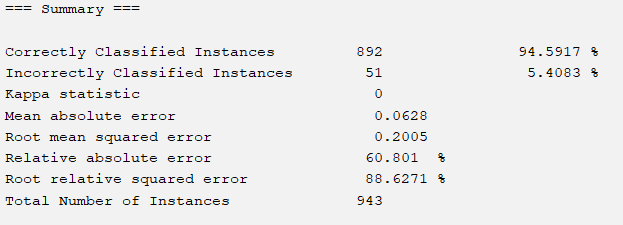
\includegraphics[width=0.5\linewidth]{b.png}
    \caption{Enter Caption}
    \label{fig:enter-label}
\end{figure}
\section{Conclusion}
The purpose of the given assignment is to study and implement Singular Value Decomposition (SVD) through practical means. Through the assignment, it was clear when SVD should and should not be applied. Furthermore, in future use cases of SVD one may want to adjust their base code or manually implement SVD to fit their specific needs.
\end{document}
